\begin{exercise}
      {ID-b14c48fd1aee3a34bcf3ba27579a9e6f9de1b7a2}
      {Tordurchfahrt}
  \ifproblem\problem
    Eine Tordurchfahrt hat die Form einer Parabel. Sie ist \simeter{6} hoch
    und \simeter{4} breit. Ein Fahrzeug ist \simeter{3} breit und \simeter{2.20}
    hoch. Kann dieses Fahrzeug die Tordurchfahrt passieren?
  \fi
  \ifoutline\outline
    \begin{minipage}{3.5cm}
      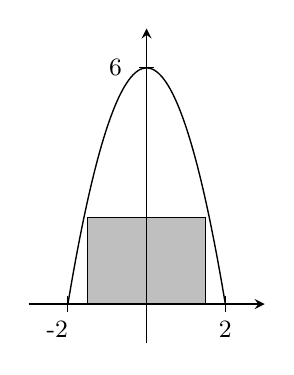
\begin{tikzpicture}[scale=0.5]
        % Fahrzeug
        \filldraw[fill=black!25!white] (-1.500, 0) rectangle (1.500, 2.200);
        % x-Achse
        \draw[->, >=stealth, line width=0.6pt] (-3.000, 0) -- (3.000, 0);
        % y-Achse
        \draw[->, >=stealth, line width=0.6pt] (0, -1) -- (0, 7.000);
        % Parabel
        \draw[line width=0.5pt] plot[smooth] coordinates
        {
          ( -2.000,   0.000)
          ( -1.900,   0.585)
          ( -1.800,   1.140)
          ( -1.700,   1.665)
          ( -1.600,   2.160)
          ( -1.500,   2.625)
          ( -1.400,   3.060)
          ( -1.300,   3.465)
          ( -1.200,   3.840)
          ( -1.100,   4.185)
          ( -1.000,   4.500)
          ( -0.900,   4.785)
          ( -0.800,   5.040)
          ( -0.700,   5.265)
          ( -0.600,   5.460)
          ( -0.500,   5.625)
          ( -0.400,   5.760)
          ( -0.300,   5.865)
          ( -0.200,   5.940)
          ( -0.100,   5.985)
          (  0.000,   6.000)
          (  0.100,   5.985)
          (  0.200,   5.940)
          (  0.300,   5.865)
          (  0.400,   5.760)
          (  0.500,   5.625)
          (  0.600,   5.460)
          (  0.700,   5.265)
          (  0.800,   5.040)
          (  0.900,   4.785)
          (  1.000,   4.500)
          (  1.100,   4.185)
          (  1.200,   3.840)
          (  1.300,   3.465)
          (  1.400,   3.060)
          (  1.500,   2.625)
          (  1.600,   2.160)
          (  1.700,   1.665)
          (  1.800,   1.140)
          (  1.900,   0.585)
          (  2.000,   0.000)
        };
        % Beschriftung
        \draw (-2.000,  0.2) -- (-2.000, -0.2) node[below]{{\small\num{-2}\hphantom{ --}}};
        \draw (2.000,  0.2) -- (2.000, -0.2) node[below]{{\small\num{2}}};
        \draw ( 0.2, 6.000) -- (-0.2, 6.000) node[left=0.25em]{{\small\num{6}}};
      \end{tikzpicture}
    \end{minipage}%
    \hspace*{\fill}%
    \begin{minipage}{11cm}
      Eine nach unten geöffnete Parabel mit dem Nullstellen \num{-2} und \num{2} hat die Form:
      \begin{equation*}
        f(x)=-(x+2)(x-2)=-(x^2-4)=-x^2+4
      \end{equation*}

      Um den Scheitelpunkt $(0\mid6)$ zu erreichen muss die Parabel noch um den Faktor \num{1.5}
      gestreckt werden:
      \begin{equation*}
        f(x)=-\num{1.5}\cdot(x^2-4)=-\num{1.5}x^2+6
      \end{equation*}
    \end{minipage}%
  \fi
  \ifoutcome\outcome
    \begin{equation*}
      f(\num{1.5})=-\num{1.5}\cdot\num{1.5}^2+6=\num{2.625}
    \end{equation*}
    Die Höhe des Torbogens \simeter{1.50} links und rechts der Mitte beträgt
    \simeter{2.625}, d.\,h. das \simeter{2.20} hohe Fahrzeug passt hindurch.
  \fi
\end{exercise}
